\documentclass[a4paper,11pt]{report}


\usepackage[german]{babel}        % Deutschsprachige Beschriftungen
\usepackage[utf8]{inputenc}       % Utf8 Zeichensatz
\usepackage[T1]{fontenc}          % Schriftenkodierung
\usepackage[lighttt]{lmodern}     % Schriftart
\usepackage{amsmath}  
\usepackage{amsfonts}            % Mathematische Formeln
\usepackage[normalem]{ulem}       % Durchgestrichener Text
\usepackage{xcolor}               % Farbiger Text
\usepackage{verbatim}             % Text ohne Formatierung
\usepackage{listings}             % Code mit Formatierung
\usepackage{csquotes}             % Kontextsensitive Zitatanlage
\usepackage{caption}              % Erweiterte Beschriftungen
\usepackage{subcaption}           % Unterbeschriftungen
\usepackage{geometry}             % Seitenränder
\usepackage{setspace}             % Zeilenabstand
\usepackage{fancyhdr}             % Header und Footer
\usepackage{graphicx}             % Grafiken
\usepackage{wrapfig}
\usepackage{float}
\usepackage{longtable}	
\usepackage{svg}                  % SVG Grafiken
\usepackage{booktabs}             % Tabellen
\usepackage{tabularx}             % Breite von Boxen
\usepackage[backend=biber, style=apa]{biblatex} % Referenzen
\usepackage[hidelinks]{hyperref}             % Hyperlinks im PDF-Dokument
\usepackage{hyperxmp}             % Metadaten im PDF-Dokument
\usepackage{makeidx}              % Optional, für Glossar (Index)
\usepackage{siunitx}   

\title{Die experimentelle Bestimmung der Elementarladung}
\date{\today}
\author{Samuel Egli}
\makeatletter            % Erlaubt das Auslesen der obigen Eigenschaften
\let\papertitle\@title   % Titel in \papertitle speichern
\let\paperdate\@date     % Datum in \paperdate speichern
\let\paperauthor\@author % Autor in \paperauthor speichern
\makeatother
\def\paperinstitution{Kantonsschule am Burggraben}
\def\papertype{Maturaarbeit}
\def\papersupervisor{Dr. Rheinhard Gross}

% ======== START VON SEITENRÄNDER ========= (Seitenränder)
\geometry{
	a4paper,
	total={150mm,237mm},
	left=30mm,
	top=30mm,
}
\setlength{\headheight}{14pt}
% ========= ENDE VON SEITENRÄNDER =========


\addbibresource{literature.bib}

\begin{document}
	
\begin{titlepage}
	\centering
	
\includegraphics[width=.3\textwidth]{title_logo.pdf}\\[.25cm]
	{\scshape\paperinstitution\par}
	\vspace{1cm}
	{\scshape\Large\papertype\par}
	\vspace{1.5cm}
	{\huge\bfseries\papertitle\par}
	\vspace{2cm}
	{\Large Vorgelegt durch:\par\paperauthor\par}
	\vfill
	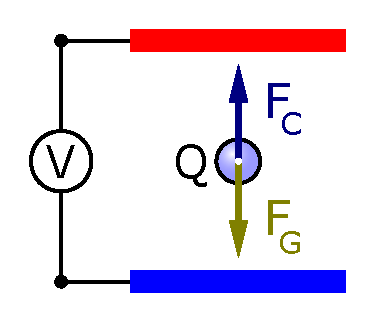
\includegraphics{titelbildMaturaarbeit.pdf}
	\vfill
	Vorgelegt bei:\par
	{\sc\papersupervisor\par}
	\vspace{0.5cm}
	{\large\paperdate\par}
	\vfill
	{\footnotesize Bildquelle: \cite[CC-BY-SA 4.0]{wiki:xxx}}
\end{titlepage}
	
	% === INHALTSVERZEICHNIS ===
	\tableofcontents %          \
	\newpage %                  \
	% --------------------------
	
	% =========== START VON STYLING ===========
	\onehalfspacing % Zeilenabstand 1.5
	\renewcommand{\chaptermark}[1]{\markboth{\MakeUppercase{\thechapter.\ #1}}{}} % Kapitel
	\renewcommand{\sectionmark}[1]{\markright{\thesection.\ #1}{}} % Abschnitt
	\fancyhead[R]{\rightmark}
	\fancyhead[L]{\leftmark}
%	\fancyhead[C]{\thepage{}} % Seitennummer
	\fancyhead[L]{\leftmark}
	\fancyhead[R]{\rightmark}
	\fancyfoot[C]{\thepage{}}
	\pagestyle{fancy}
	% =========== ENDE VON STYLING ============
	
	\chapter{Einführung}\label{ch:einfuerung}
\section{Einleitung}\label{sec:einleitung}
Warum wird ein Draht heiss wenn Strom durchfliesst? Kann das mit dem Aufladen eines Handys verglichen werden? Ja, in beiden Fällen verursacht die Reibungsenergie der Elektronen die thermische Veränderung des Drahtes. Physikalisch gesehen ist der Fluss von geladenen Teilchen alltagsprachlich definiert als elektrischen Strom.
  
Stellen Sie sich vor, Sie untersuchen die kleinsten geladenen Teilchen, die man bisher kennt. Sie erhalten sehr genaue Messwerte und glauben, die Natur der Elementarladung erforscht zu haben. Sie veröffentlichen Ihre Arbeit, aber eifersüchtige Konkurrenten versuchen Sie niederzumachen, indem sie behaupten, Sie hätten Messwerte ausgeschlossen, die nicht stimmten.  Diesen Konkurrenten versuchen sie zu beweisen, dass das, was Sie erforscht haben, wahr ist. Es vergeht eine lange Zeit, bis Sie dies beweisen können. Etwa 13 Jahre später gewinnen Sie mit Ihrer Entdeckung der Elementarladung den Nobelpreis für Physik. Sie haben genau das durchgemacht, was Robert Andrews {\scshape Millikan} in den Jahren des Ersten Weltkrieges durchgemacht hat.

Diese Arbeit soll zeigen, wie man zu Beginn des 20. Jahrhunderts ein solches Experiment erfunden hat, wie man vor mehr als hundert Jahren so genaue Messwerte erhalten hat und wie genau solche Messungen sind, wenn man das Experiment heute durchführt.

% Quelle: https://de.wikipedia.org/wiki/Robert_Andrews_Millikan

\section{Biographie von Millikan}\label{sec:autobiographie}
Robert Andrews {\sc Millikan} wurde 1868 in Amerika geboren. Im Alter von 18 Jahren begann er am Oberlin College in Ohio zu studieren. Zunächst studierte er Mathematik und Griechisch, später belegte er einen Kurs in Physik und legte sein Examen als Physiklehrer ab. Etwa 10 Jahre später promovierte er an der Columbia University. Nach seiner Promotion ging er für ein Jahr nach Deutschland, um seine Kenntnisse bei Max {\sc Planck} und Walther {\sc Nernst} zu vertiefen. Danach kehrte er in die USA zurück, wo er 10 Jahre als Professor an der University of Chicago arbeitete. 

1909 begann er, die Natur der Elementarladung zu erforschen. Anfangs benutzte er die \textit{Tröpfchenmethode}, die mit Wasser durchgeführt wurde. Später benutzte er die \textit{Öltröpfchenmethode}, die für die Bestimmung der Elementarladung besser geeignet war, da sich Öltröpfchen im Vergleich zu Wassertröpfchen als stabiler erwiesen.  Mit dieser Methode gelang es ihm, die Einheit der kleinsten elektrischen Ladung zu bestimmen, die er mit $e$ bezeichnete. Ein Jahr später veröffentlichte er seine Arbeit mit mehr als 38 Messungen. Sie stieß bei anderen Forschern auf grosses Interesse, aber auch auf heftige Kritik. Um die Kritik zu entkräften, veröffentlichte er drei Jahre später eine weitere Arbeit über die experimentelle Bestimmung der Elementarladung, doch auch diese Ergebnisse wurden angezweifelt. In den Jahren vor dem Ersten Weltkrieg erhielt er 3-4 Auszeichnungen, darunter den Comstock-Preis für Physik.

Millikan untersuchte nicht nur die Natur der Elementarladung, sondern wollte auch die Lichtquantenhypothese von Albert {\sc Einstein} experimentell überprüfen, da er Einsteins Interpretation skeptisch gegenüberstand. Es gelang ihm jedoch, die Richtigkeit von Einsteins Gleichungen zu beweisen.

Als Millikan 1918 sein Buch "Das Elektron" veröffentlichte, behauptete er, seine Messungen der Elementarladung seien genauer als die seiner Konkurrenten, da die Werte nur wenig streuten. Diese Arbeit begründete seinen späteren Ruhm und die Verleihung des Nobelpreises im Jahr 1923. 

In der Zwischenkriegszeit setzte er seine Forschungen fort, bis er 1946 in den Ruhestand trat. Er schrieb zahlreiche Bücher über Natur und Religion sowie verschiedene Lehrbücher. %\parencite[vgl.][Millikan]{dewiki:247237013}

\section{Relevanz der Elementarladung Heute}\label{sec:relevanz}
In welchen Bereichen des täglichen Lebens benötigen wir heute Elementarladungen? Die wohl bekannteste Technik, bei der wir reine Elementarladungen (Elektronen) benötigen, ist die Röntgentechnik in der Medizin. Ein Röntgengerät ist nichts anderes als ein Teilchenbeschleuniger, der Elektronen auf den bzw. durch den Körper schiesst. Ein anderes Beispiel aus der Medizin ist das Bestrahlungsgerät in der Krebstherapie. Hier werden keine Elektronen, sondern Protonen mit genau der gleichen Ladung, $1.602176634 \cdot 10^{-19} C$ \parencite[123]{fundamentum_mathe}, aber positiv statt negativ, beschleunigt und auf den Körper geschossen. 

Ohne das Wissen, dass es keine Ladung gibt, die kleiner als die Elementarladung ist, würde heute keines unserer elektronischen Geräte, insbesondere keine elektronischen Rechner, funktionieren. Denn jedes Bit in unseren Chips basiert darauf, ob ein Elektron fehlt oder nicht.

Um die Masse eines Elektrons zu bestimmen, benötigt man auch die Elementarladung \textit{e}. Mit Hilfe eines Magneten wird ein Elektron auf eine Kreisbahn geschickt. Dabei wirkt auf das Elektron eine magnetische Kraft (Lorentzkraft). Um eine Kreisbewegung zu erzielen, braucht es eine Zentripetalkraft, die von der Lorentzkraft aufgebracht wird. Formal ausgedrückt bedeutet das: $F_L \ = \ F_Z$, wobei $F_L \ = \ e \cdot v \cdot B$. Dabei steht $e$ für die Elementarladung

   

	\chapter{Theoretische Grundlagen}\label{ch:theorieGrundlagen}
\section{Elementarladung}\label{sec:elementarladung}
\subsection{Definition}\label{sub:definition}
Die Elementarladung wird physikalisch definiert als,

\begin{equation}\label{eq:definition}
 q  =  n \cdot e \:  \Leftrightarrow \: e = \frac{q}{n} \quad | \ n \in \mathbb{Z}
\end{equation}

\noindent Diese Definition bedeutet nichts anderes, als dass alle möglichen Ladungen ganzzahlige Vielfache der Elementarladung $e$ sind. Diese Erkenntnis bekommt man über den Millikan-Versuch, der aufzeigt, dass sich die Ladungen von Körpern nicht kontinuierlich verteilen, sondern nur in Etagen vorkommen. 

Die Elementarladung besitzt die Einheit Coulomb C. Sie steht als Einheitssymbol für die physikalische Grösse der Ladung $[Q]$. Manchmal wird anstatt Coulomb auch die alternative Schreibweise, die Amperesekunde, verwendet. Das soll Sie aber nicht verwirren, denn die Einheit Coulomb setzt sich aus dem Ampere $[I]$ und der Zeit $[t]$ zusammen. Formal ausgedrückt bedeutet dass: $I \cdot t = Q$. 

\subsection{Eigenschaften}\label{sub:eigenschaften}
Wie oben in \autoref{sec:elementarladung} hergeleitet, hat die Elementarladung die Eigenschaft, dass sie die kleinst mögliche Ladungseinheit in der Natur ist. Kontrovers wird es wenn man Ihnen jetzt sagt das auch drittel Elementarladungen möglich sind. Ein Proton, das die Ladung 1e beträgt, besteht aus drei kleinsten Elementarteilchen, den Quarks. Quarks sind die kleinsten im Moment bekannten Elementarteilchen und sie sind die Bausteine der Materie. Es gibt verschiedene Arten von Quarks, wir beschäftigen uns aber nur mit den Up und Down Quarks. Das Proton besteht aus zwei Up-Quarks und einem Down-Quark. in der folgenden \autoref{tab:quark_tabelle} kann man die verschiedenen Ladungen der Quarks sehen. Wenn man diese Ladungen nun zusammenrechnet kommt man wieder auf die Elementarladung e. 

\begin{equation}\label{eq:mathematische_zusammensetzung_von_qurks}
	2 \cdot \left(\frac{2}{3}e\right)  + 1 \cdot \left( -\frac{1}{3}e\right) 
	= \frac{4}{3}e - \frac{1}{3}e = 1e
\end{equation}

\noindent Wie in \autoref{eq:mathematische_zusammensetzung_von_qurks} gezeigt, kann die Elementarladung auch aus Bruchteilen von sich selber bestehen. Wieso hat man jetzt genau die Ladung eines Elektron oder Proton als Elementarladung festgelegt? Das ist sehr einfach zu beantworten, wenn man die Verhaltensweise von Quarks kennt. Quarks kommen nie einzeln in der Natur von, sondern nur in sogenannten Quark-Gluon-Plasmen. Einfach ausgedrückt nur als Pärchen in einem Proton oder Neutron.

%\begin{figure}[h]\label{fig:quarkTabelle}
	%\begin{center}
		%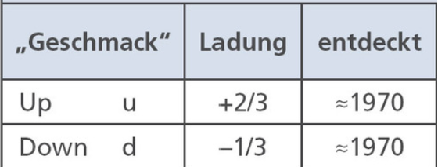
\includegraphics[scale=1]{bilder/pdf/quark_tabelle.pdf}
	%	\caption{Tabelle Ladung von Quarks}
%	\end{center}
%\end{figure}

\begin{table}[ht]
	\begin{center}
		\begin{tabular}{l|l}
			\multicolumn{2}{c}{\textit{\textbf{Quark Tabelle}}} \\
			\hline
			Art & Ladung \\
			\hline
			Up u & $+ \frac{2}{3}e$ \\
			\hline
			Down d & $- \frac{1}{3}e$\\
			\hline
		\end{tabular}
	\end{center}
	\caption{Up-Down-Quark Ladungen}
	\label{tab:quark_tabelle}
\end{table}

\section[Historische Methoden]{Historische Methoden zur Bestimmung der Elementarladung}
\subsection{Thomsonsche Methode}\label{sub:thomson}
In dieser Arbeit geht es hauptsächlich um den Millikan-Versuch, zur Bestimmung der Elementarladung. Andere Methoden sind aber dennoch nennenswert. Zum Beispiel das Thomsonsche Experiment. Dabei geht es um einen Versuch, der ein Elektronenstrahl durch ein magnetisches Feld schiesst. Dabei wird der Strahl durch die Lorenzkraft abgelenkt und Joseph John {\scshape Thomson} konnte, durch verändern des Magnetfeldes, das Verhältnis von Masse und Ladung $\frac{e}{m}$ entdecken. Durch dieses Verhältnis konnte er die Elementarladung noch nicht bestimmen. Erst später als man die Masse eines Elektron entdeckte, konnte man indirekt über dieses Verhältnis auf die Ladung zurückschliessen. 

\subsection{Elektrolyse}\label{sub:elektrolyse}
Eine andere Methode, die Elementarladung zu ermitteln, funktioniert mithilfe der Elektrolyse. Bei der Elektrolyse wird eine Spannung angelegt um chemische Reaktionen (zum Beispiel Zersetzung von Molekülen) in einer ionischen Lösung zu erzwingen. Dabei kann man durch Messungen der Spannung und Anzahl Ionen, die gewandert sind, auf die Elementarladung schliessen. 

Mit beiden dieser Methoden kann man die Elementarladung indirekt bestimmen. Sie sind für diese Arbeit sicher nennenswert, jedoch kann man mithilfe des Millikan Versuchs viel direkter Ladungen kleinster Partikel messen.

\section{Theorie des Versuchs}\label{sec:versuchsTheorie}
Da wir die anderen Methoden nur kurz angeschnitten haben, wird der Millikan Versuch jetzt genauer erklärt oder zumindest die Theorie dahinter. 

Wir beginnen mit einem Öltröpfchen im Freien Fall. Folgende \autoref{fig:freierFall} ist dazu zu sehen.

\begin{figure}[h]
	\begin{center}
		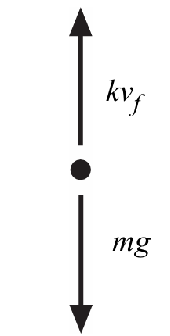
\includegraphics[scale=0.5]{bilder/pdf/Abbildung1_FreierFall.pdf}
		\caption{Öltröpfchen im Freien Fall}
		\label{fig:freierFall}
	\end{center}
\end{figure}

\noindent In \autoref{fig:freierFall} sehen wir welche Kräfte auf ein Öltröpfchen im freien Fall wirken. Nach unten haben wir die Gewichtskraft, die Abhängig ist von der Masse \textbf{$m$} und dem Ortsfaktor \textbf{$g$}. Das Öltröpfchen fällt in der Luft und hat seine Endgeschwindigkeit erreicht (die dazu benötigte Zeit beträgt wenige Millisekunden). Die Kraft, die nach oben zeigt, ist die Reibungskraft der Luft. Sie ist abhängig von der Fall- bzw. Endgeschwindigkeit \textbf{$v_f$} und dem Reibungskoeffizienten \textbf{$k$} von Luft und dem Tröpfchen.
Diese Kräfte sind genau gleich gross, weil sie in einem Kräftegleichgewicht sind. 

\begin{equation}\label{eq:kräfteFreierFall}
	mg \ = \ kv_f
\end{equation}   

\noindent Nun setzen wir dieses Öltröpfchen in ein elektrisches Feld. Mit den Kräftevektoren eingezeichnet, sieht das so aus.

\begin{figure}[h]
	\begin{center}
		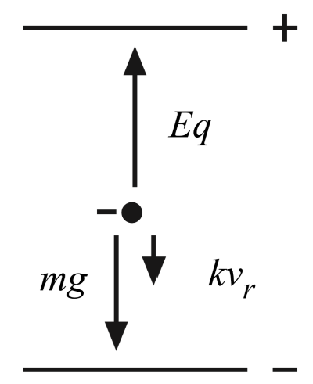
\includegraphics[scale=0.5]{bilder/pdf/Abbildung2_elektrischesFeld.pdf}
		\caption{Öltröpfchen im elektrischen Feld}
		\label{fig:elektrischesFeld}
	\end{center}
\end{figure}

\noindent Die elektrische Kraft, die in \autoref{fig:elektrischesFeld} nach oben zeigt, ist abhängig von der elektrischen Feldstärke $E$ und der Ladung $q$ des Tröpfchen. Da die elektrische Kraft nun grösser als die Gewichtskraft ist, steigt das Tröpfchen. Wie wir schon oben im Freien Fall behandelt haben, gibt es wieder eine Reibungskraft der Luft die entgegengesetzt der Bewegungsrichtung verläuft. Dieses Mal ist sie aber nicht von der Fallgeschwindigkeit abhängig, sondern von der Steiggeschwindigkeit $v_r$ (steig auf Englisch: rise) und wie oben von dem Reibungskoeffizienten der Luft $k$. Wenn man jetzt diese Vektoren algebraisch addiert, kommt man auf folgende Gleichung.

\begin{equation}\label{eq:elektrischesFeld}
	Eq \ = \ mg \cdot kv_r
\end{equation}

\noindent Nun kann man nach $q$ umstellen und den Reibungskoeffizienten $k$ mithilfe der \autoref{eq:kräfteFreierFall} eliminieren. 

\begin{equation}\label{eq:hauptgleichung}
	q \ = \ \frac{mg \cdot (v_f + v_r)}{Ev_f}
\end{equation}

\noindent Die Masse eines Öltröpfchens zu bestimmen, ist in diesem Fall fast unmöglich. Aus diesem Grund versucht man über die Dichte des Öls $\rho$, und das Volumen der Ölkugel, auf die Masse zu kommen. Der Zusammenhang von Dichte und Masse sieht folgendermassen aus: $\rho \ = \ \frac{m}{V} \ \Leftrightarrow \ m \ = \ \rho \cdot V$. Das Volumen kann jetzt noch ausgerechnet werden mithilfe des Radius $a$. Setzt man nun alles zusammen, kommt man auf folgende Formel für die Masse eines Öltröpfchens. 

\begin{equation}\label{eq:masseFormel}
	mg \ = \ \frac{4}{3} \pi a^3 \rho g
\end{equation}

\noindent Wir können jetzt dieses $m$ mit dem $m$ in \autoref{eq:hauptgleichung} substituieren.

\begin{equation}\label{eq:ladungFormel}
	q \ = \ \frac{4\pi a^3\rho g (v_f + v_r)}{3(Ev_f)}
\end{equation}

\noindent Das neue Problem wird jetzt der Radius $a$ sein. Die Tröpchen sind zu klein, um den Radius zu messen. Die Lösung des Problems finden wir im stokesschen Reibungsgesetz $(F_f \ = \ 6\pi \eta a v_f)$. Es zeigt den Zusammenhang von Fallgeschwindigkeit und Reibungskraft der Luft. Diese Formel beschreibt, wie sich ein Kugelförmiges Objekt in einem viskosem Medium verhält. Dieses Gesetz hängt von der Reibungszahl der Luft $\eta$ und der Fallgeschwindigkeit $v_f$ ab. Wir können diesen Ausdruck mit dem rechten Ausdruck von Gleichung \ref{eq:masseFormel} gleichsetzen. Wenn man nach $a$ auflöst erhält man:

\begin{equation}\label{eq:stokesRadius}
	a \ = \ \sqrt{\frac{9\eta v_f}{2\rho g}}
\end{equation}

\noindent Das stokessche Reibungsgesetz wird leider inkorrekt wenn die Fallgeschwindigkeit weniger als 0.1 cm/s beträgt. Da wir es im Experiment mit Fallgeschwindigkeiten zwischen 0.01 und 0.001 cm/s (zwischen $10^-4$ und $10^-6$ m/s) zu tun haben, müssen wir das Reibungsgesetz mit einem Korrekturfaktor multiplizieren. Die effektive Viskosität resultiert aus:

\begin{equation}\label{eq:effViskosität}
	\eta_{eff} \ = \ \eta \left( \frac{1}{1 + \frac{b}{pa}} \right) 
\end{equation}

\noindent $b$ ist dabei eine Konstante und $p$ ist der atmosphärische Druck in Pascal. 

\noindent Nun wird $\eta_{eff}$ in Gleichung \ref{eq:effViskosität} für $\eta$ in Gleichung \ref{eq:stokesRadius} substituiert. 

\begin{equation}\label{eq:korrekturRadius}
	a \ = \ \sqrt{\frac{9\eta v_f}{2\rho g} \left( \frac{1}{1 + \frac{b}{pa}}\right)}
\end{equation}

\noindent \autoref{eq:effViskosität} enthält den Radius $a$. Das Problem ist, dass wir einen Term für $a$ gefunden haben, der $a$ aber enthält. Der Ausdruck für $a$ in \autoref{eq:korrekturRadius} kann in eine quadratische Gleichung umgewandelt werden:

\begin{equation}\label{eq:quadraticRadius}
	\begin{split}
		a & \ = \ \sqrt{\frac{9\eta v_f}{2\rho g} \left( \frac{1}{1 + \frac{b}{pa}}\right)} \\
		a^2 & \ = \ \frac{9\eta v_f}{2\rho g} \left( \frac{1}{1 + \frac{b}{pa}}\right) \\
		a^2 + \frac{b}{p}a & \ = \ \frac{9\eta v_f}{2\rho g} \\
		a^2 + \frac{b}{p}a - \frac{9\eta v_f}{2\rho g} & \ = \ 0
	\end{split}
\end{equation} 

\noindent Jetzt wird \autoref{eq:quadraticRadius} nach $a$ aufgelöst:

\begin{equation}\label{eq:qRadius}
	a \ = \ \sqrt{\left( \frac{b}{2p}\right)^2 + \frac{9\eta v_f}{2\rho g}} - \frac{b}{2p}
\end{equation}

\noindent Es ist zu beachten, dass, nicht wie bei \autoref{eq:korrekturRadius}, jetzt kein $a$ im Ausdruck mehr vorkommt. Jetzt wird der komplette Term für $a$ in Gleichung \ref{eq:ladungFormel} ersetzt.

\begin{equation}\label{eq:ladungMitEingesetzR}
	q \ = \ \frac{4\pi \left[ \sqrt{\left( \frac{b}{2p}\right)^2 + \frac{9\eta v_f}{2\rho g}} - \frac{b}{2p} \right]^3 \rho g(v_f + v_r) }{3(Ev_f)}
\end{equation}

\noindent Die Elektrische Feldstärke $E$ kann auch so ausgedrückt werden:

\begin{equation}\label{eq:elektrischeFeldstärke}
	E \ = \ \frac{V}{d}
\end{equation}

\noindent Wenn jetzt $E$ aus Gleichung \ref{eq:ladungMitEingesetzR} mit $E$ aus \autoref{eq:elektrischeFeldstärke} ersetzt wird und die ganze Gleichung noch schöner umgeformt wird, resultiert daraus:

\begin{equation}\label{eq:letzteFormel}
	q \ = \ \frac{4\pi}{3} \cdot \left[ \sqrt{\left( \frac{b}{2p}\right)^2 + \frac{9\eta v_f}{2\rho g}} - \frac{b}{2p} \right]^3 \cdot \frac{\rho gd(v_f + v_r)}{Vv_f}
\end{equation}

\noindent Die Quelle für all diese Berechnungen basieren auf \parencite{instructionManual}




	


	\chapter{Experimenteller Aufbau}\label{cha:experimentAufbau}
\section{Versuchsanordnung}\label{sec:versuchsanordnung}

Wie bereits in \autoref{sec:versuchsTheorie} erläutert, basiert das Millikan-Experiment auf dem Kräftegleichgewicht zwischen der Gewichtskraft und der elektrischen Kraft. Zu Beginn wird ein dunkler Raum benötigt, wobei eine Dunkelkammer, in der keinerlei äusseres Licht eindringen kann, ideal ist. Das einzige Licht, das während des Experiments verwendet wird, stammt aus einem Mikroskop, das am Experimentapparat angebracht ist.

Während des Versuchs werden sehr kleine Öltröpfchen mithilfe eines Zerstäubers in eine Kammer eingebracht. Die Fallgeschwindigkeit der Tröpfchen wird anschliessend durch Beobachtung mit dem Mikroskop und anhand des Lichts gemessen.

Der Boden als auch die Decke bestehen aus elektrisch geladenen Kondensatoren, was es ermöglicht, ein elektrisches Feld zu erzeugen. Über einen Schalter kann die Richtung des elektrischen Feldes verändert werden. Diese Funktion wird insbesondere bei der zweiten Messung benötigt, bei der die Kondensatoren aktiviert werden, sodass das elektrische Feld nach oben gerichtet ist (Decke + Boden -). Wenn die Öltröpfchen negativ geladen sind, können sie die Gravitationskraft überwinden und steigen nach oben. Die Geschwindigkeit, die die Tröpfchen benötigen, um von einer Gitterlinie zur nächsten zu gelangen, wird dabei erneut gemessen. Dieser Vorgang wird wiederholt, bis das Tröpfchen nicht mehr sichtbar ist. Eine detaillierte Schritt-für-Schritt-Anleitung wird in \autoref{sec:durchfuehrung} bereitgestellt.

\section{Material}\label{sec:material}

In dieser Arbeit wurde das \textit{Model AP-8210 von PASCO scientific} mit der Halogenlampe verwendet. \\

\noindent \textbf{Material, das dabei ist:}

\begin{itemize}
	\item Apparat Plattform und Kondensator Ladungsschalter (Eine genauere Beschreibung der Plattform in \autoref{sub:inhaltApparatur})
	\item 12 Volt DC Transformator für die Halogenlampe
	\item nicht flüchtiges Öl
	\item Ölsprüher 
\end{itemize}

\subsection{Plattform}\label{sub:inhaltApparatur}
Da das Experiment bereits vollständig aufgebaut ist, werden im Folgenden alle Komponenten aufgezählt, die sich auf der Plattform befinden.

\noindent \textbf{Komponenten der Plattform:}

\begin{itemize}\label{item:apparatur}
	\item Tröpfchenbetrachtungskammer (Wird im nächsten \autoref{sub:viewingChamber})
	\item Betrachtungsfernrohr (30X, Hellfeld, aufrechtes Bild) mit Fadenkreuz (Linienabstand: 0,5 mm grosse Teilung, 0,1 mm kleine Teilung), Fadenkreuz-Fokussierring und Tropfenfokussierring
	\item Halogenlampe (12 V, 5 W)
	\item Fokussierdraht
	\item Kondensatorenspannungsanschlüsse
	\item Thermistoranschlüsse (sind an den unteren Kondensator eingebaut)
	\item Thermistortabelle (Widerstand-Temperatur)
	\item Ionisationsquellenschalter (3 verschiedene Positionen: Ionisation AN, Ionisation AUS, Sprühposition)
	\item Wasserwaage
	\item Kondensatorladungsschalter (mit einem Meter Kabel, um Vibrationen zu vermeiden)
\end{itemize}


\subsection{Betrachtungskammer}\label{sub:viewingChamber}
Die Betrachtungskammer ist zerlegbar. Die einzelnen Komponenten werden im Folgenden aufgelistet.

\noindent \textbf{Einzelteile der Betrachtungskammer:}

\begin{itemize}\label{item:betrachtungskammer}
	\item Deckel
	\item Gehäuse
	\item Tröpfchenlochabdeckung
	\item obere Kondensatorplatte
	\item Abstandshalter aus Plastik (ungefähr 7.6mm dick)
	\item untere Kondensatorplatte
	\begin{itemize}
		\item Thorium-232 Alphateilchenquelle
		\item elektronische Verbindung zur oberen Platte
	\end{itemize}
	\item konvexe Linse
\end{itemize}

\begin{figure}[h]
	\centering
	\begin{minipage}[t]{0.45\textwidth}
		\centering
		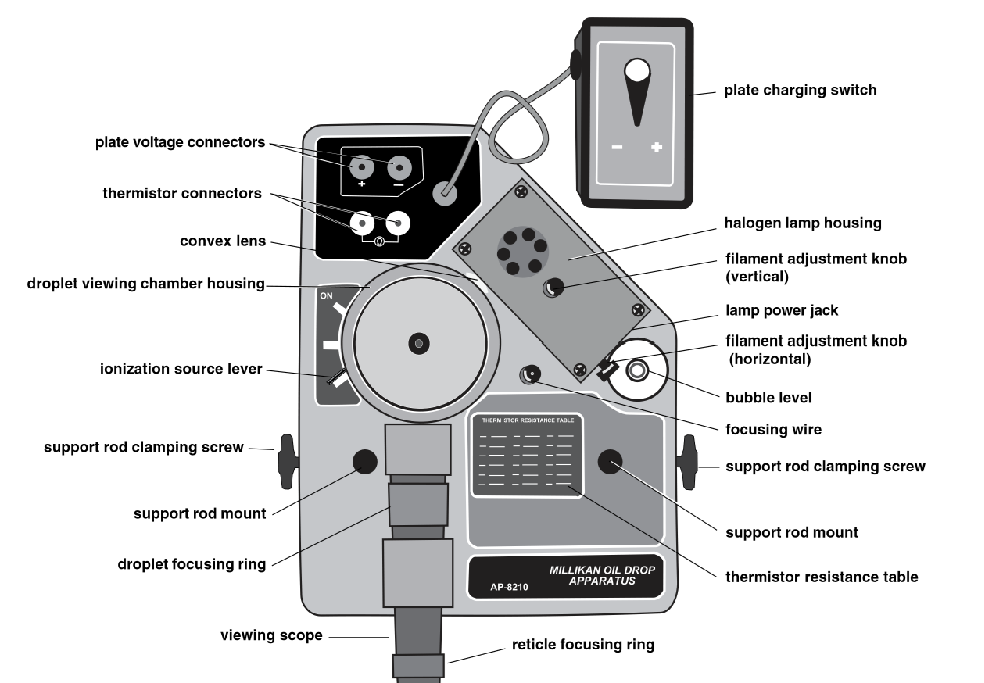
\includegraphics[scale=0.5]{bilder/pdf/plattformKomponenten.pdf}
		\caption{Komponenten der Plattform \parencite[3]{instructionManualHalogen}}
		\label{fig:plattformKomp}
	\end{minipage}
	\hfill
	\begin{minipage}[t]{0.45\textwidth}
		\centering
		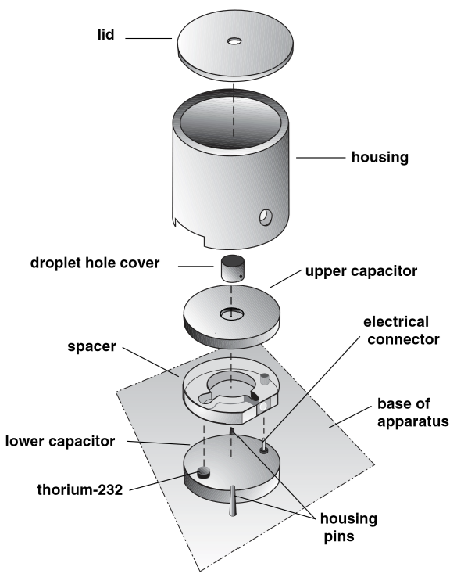
\includegraphics[width=\textwidth]{bilder/pdf/BetrachtungsKammerKomponenten.pdf}
		\caption{Komponenten der Betrachtungskammer \parencite[4]{instructionManualHalogen}}
		\label{fig:betrachtKomp}
	\end{minipage}
\end{figure}

\noindent Das gesamte Material ist in einem Experimentierkasten enthalten. Dieses Experiment wurde von der Kantonsschule am Burggraben für die Durchführung dieser Arbeit zur Verfügung gestellt.






	\chapter{Durchführung}\label{cha:durchfuehrung}
	\chapter{Auswertung}\label{cha:auswertung}
\section{Ausgehobene Daten}\label{sec:aushebungDaten}
Dieses Kapitel befasst sich mit der Genauigkeit der Bestimmung der Elementarladung. Zunächst wird ein Blick auf die im Experiment erhaltenen Daten geworfen. In \autoref{tab:ergebnisse} sind die relevanten Messgrößen aufgeführt, nämlich die Steig- und Fallgeschwindigkeiten, der Radius, die Masse sowie die Ladung der Tröpfchen. Eine vollständige Übersicht der Messwerte ist im Anhang zu finden, wobei auch Messungen, die nicht ausreichend präzise waren, berücksichtigt werden. Diese wurden in den Berechnungen jedoch nicht einbezogen.

Die Daten können nun in einem Punktdiagramm visualisiert werden, wobei die Y-Achse die Ladung der Tröpfchen und die X-Achse die jeweilige Nummer der Messung darstellt. Das Diagramm wurde mit Microsoft Excel erstellt und ist wie folgt dargestellt.

\begin{figure}[h]
	\centering
	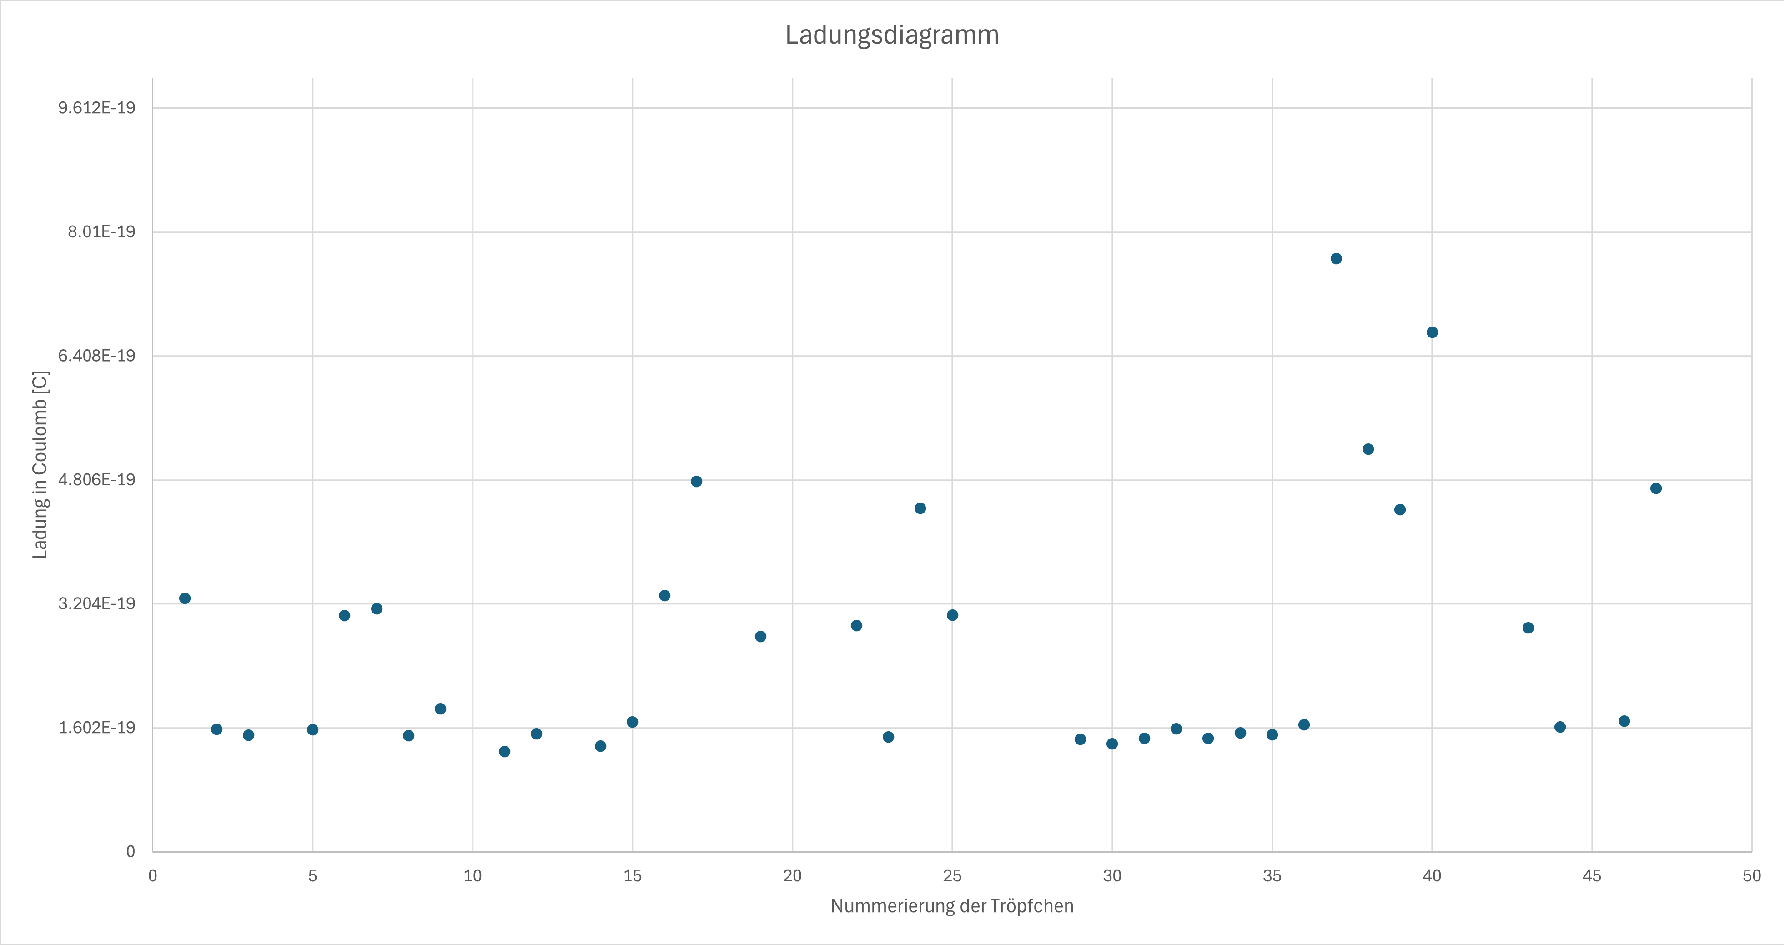
\includegraphics[width=\textwidth]{bilder/pdf/LadungsdiagrammOhne.pdf}
	\caption{Ladungsdiagramm ohne Fehlerrechnung}
	\label{fig:ladungsdiagrammOFehlerrechnung}
\end{figure}

\noindent Die Abstände auf der Y-Achse sind nicht zufällig gewählt, sondern entsprechen exakt einem Linienabstand für eine Elementarladung. Anhand dieses Diagramms kann die Anzahl der Elementarladungen jedes einzelnen Tröpfchens abgelesen werden. Es war überraschend, wie präzise das Experiment verlief. Die Ladungen der Tröpfchen ordnen sich deutlich in Stufen an, was während des Experimentierens nicht zu erwarten war. Weitere Details zur Genauigkeit der Messungen werden in \autoref{sec:genauigkeitAuswertung} behandelt, wobei eine Fehlerrechnung zur Bewertung der Resultate herangezogen wird. Während des gesamten Experimentierens und Auswertens traten keine unplausiblen Werte auf, die eine viel zu hohe oder niedrige Ladung ergaben. Dies war besonders überraschend, da das Experiment von einer Vielzahl verschiedener Faktoren und Messgrößen abhängt.

\section{Das Ergebnis}\label{sec:ergebnis}
In der \autoref{tab:ergebnisse} kann nun eine weitere Spalte eingefügt werden, die die Anzahl der Elementarladungen $n$ angibt. Nachdem diese hinzugefügt wurde, sieht die Tabelle für die ersten 10 Zeilen wie folgt aus:

\begin{table}[H]
	\centering
	\begin{tabular}{llllll|l}
		\toprule
		Nr. & $v_{rise}$ & $v_{fall}$ & Radius & Masse & Ladung & Anzahl (n) \\
		\midrule
		1 &$\mathrm{2.01 \cdot 10^{-04}}$ & $\mathrm{2.12 \cdot 10^{-05}}$ & $\mathrm{4.04 \cdot 10^{-07}}$ & $\mathrm{2.45 \cdot 10^{-16}}$ & $\mathrm{3.27 \cdot 10^{-19}}$ & 2\\
		2 &$\mathrm{8.46 \cdot 10^{-05}}$ & $\mathrm{2.16 \cdot 10^{-05}}$ & $\mathrm{4.08 \cdot 10^{-07}}$ & $\mathrm{2.53 \cdot 10^{-16}}$ & $\mathrm{1.59 \cdot 10^{-19}}$ & 1\\
		3 &$\mathrm{8.68 \cdot 10^{-05}}$ & $\mathrm{1.98 \cdot 10^{-05}}$ & $\mathrm{3.90 \cdot 10^{-07}}$ & $\mathrm{2.20 \cdot 10^{-16}}$ & $\mathrm{1.51 \cdot 10^{-19}}$ & 1\\
		4 &$\mathrm{8.91 \cdot 10^{-05}}$ & $\mathrm{2.04 \cdot 10^{-05}}$ & $\mathrm{3.96 \cdot 10^{-07}}$ & $\mathrm{2.31 \cdot 10^{-16}}$ & $\mathrm{1.58 \cdot 10^{-19}}$ & 1\\
		5 &$\mathrm{1.97 \cdot 10^{-04}}$ & $\mathrm{1.98 \cdot 10^{-05}}$ & $\mathrm{3.89 \cdot 10^{-07}}$ & $\mathrm{2.18 \cdot 10^{-16}}$ & $\mathrm{3.05 \cdot 10^{-19}}$ & 2\\
		6 &$\mathrm{1.98 \cdot 10^{-04}}$ & $\mathrm{2.04 \cdot 10^{-05}}$ & $\mathrm{3.96 \cdot 10^{-07}}$ & $\mathrm{2.31 \cdot 10^{-16}}$ & $\mathrm{3.14 \cdot 10^{-19}}$ & 2\\
		7 &$\mathrm{9.33 \cdot 10^{-05}}$ & $\mathrm{1.84 \cdot 10^{-05}}$ & $\mathrm{3.74 \cdot 10^{-07}}$ & $\mathrm{1.95 \cdot 10^{-16}}$ & $\mathrm{1.50 \cdot 10^{-19}}$ & 1\\
		8 &$\mathrm{1.26 \cdot 10^{-04}}$ & $\mathrm{1.71 \cdot 10^{-05}}$ & $\mathrm{3.61 \cdot 10^{-07}}$ & $\mathrm{1.74 \cdot 10^{-16}}$ & $\mathrm{1.85 \cdot 10^{-19}}$ & 1\\
		9 &$\mathrm{1.12 \cdot 10^{-04}}$ & $\mathrm{1.23 \cdot 10^{-05}}$ & $\mathrm{3.01 \cdot 10^{-07}}$ & $\mathrm{1.01 \cdot 10^{-16}}$ & $\mathrm{1.29 \cdot 10^{-19}}$ & 1\\
		10 &$\mathrm{1.30 \cdot 10^{-04}}$ & $\mathrm{1.29 \cdot 10^{-05}}$ & $\mathrm{3.08 \cdot 10^{-07}}$ & $\mathrm{1.09 \cdot 10^{-16}}$ & $\mathrm{1.53 \cdot 10^{-19}}$ & 1\\
		\bottomrule
		&&&&& $2.031 \cdot 10^{-18}$ & 13 \\
	\end{tabular}
	\caption{Ergebnisse mit Anzahl Ladungen}
	\label{tab:anzahlLadung}
\end{table}
\par
\noindent Die Anzahl der Elementarladungen wird addiert, was zu einer Summe von 13 Elementarladungen führt. Anschließend werden die Ladungen summiert, was den Wert $2.031 \cdot 10^{-18}$ Coulomb ergibt. Das arithmetische Mittel aus diesen beiden Messwerten lautet dann: $\frac{2.031 \cdot 10^{-18}}{13} \ = \ 1.56 \cdot 10^{-19} Coulomb$. 

Wenn dieser Vorgang für alle Werte in der Tabelle wiederholt wird, ergibt sich eine Anzahl von 60 Elementarladungen und eine Gesamtsumme von $9.313 \cdot 10^{-18}$ Coulomb. Das Mittel dieser Werte führt zu einem Ergebnis für die Elementarladung von:

\begin{equation}\label{eq:ergebnis}
	\frac{9.313 \cdot 10^{-18}C}{60} \ = \ 1.552 \cdot 10^{-19} Coulomb
\end{equation}

\section{Die Genauigkeit}\label{sec:genauigkeitAuswertung}
Die Genauigkeit eines solchen Experimentes kann nur durch eine gründliche Fehleranalyse bewertet werden. Im Folgenden wird die Fehlerrechnung erläutert, um den Einfluss der Fehlerquellen auf das Ergebnis zu quantifizieren. Für jede relevante Größe wird sowohl der absolute als auch der relative Fehler berechnet, wobei diese Fehler anschließend miteinander kombiniert werden, um die Gesamtunsicherheit der Messergebnisse zu ermitteln.

In jedem Experiment treten Fehler auf, die entweder durch die Messinstrumente oder durch den Experimentieraufbau verursacht werden. Ein Beispiel für solche systematischen Fehler ist die mögliche Fehlausrichtung des Multimeters oder eine ungenaue Gitterabmessung, bei der die Gitternetzlinien nicht exakt 0,5 mm voneinander entfernt sind. Systematische Fehler können durch präzise Kalibrierung der Geräte und sorgfältige Vorbereitung des Experiments minimiert oder, wenn möglich, vollständig vermieden werden.

Zusätzlich gibt es auch zufällige Fehler, die durch unkontrollierbare Schwankungen während des Experiments auftreten. Beispiele hierfür sind die Reaktionszeit beim Starten der Stoppuhr, der Blickwinkel beim Beobachten der Tröpfchen oder auch Umweltfaktoren wie Temperatur- und Luftdruckschwankungen während des Experiments. Diese Fehler sind schwieriger zu eliminieren, können jedoch durch wiederholte Messungen und die Berechnung von Mittelwerten verringert werden, wodurch der Effekt der zufälligen Fehler minimiert wird.

\subsection{Fehlerrechnung}\label{sub:fehler}
Zuerst müssen für alle Messgrössen absolute Fehler entschieden werden. Die können abgeschätzt werden oder hängen von der Genauigkeit eines Messgerätes ab.

\begin{table}[h]
	\begin{center}
		\begin{tabular}{l|lll}
			                             & Messwert     & absoluter Fehler     & relativer Fehler [\%] \\ \toprule
			Elektrisches Feld $[V/m]$    & zsmg. Grösse &                      & 0.68\%                \\
			Steigzeit $[s]$              & 3.7          & 0.1                  & 2.70\%                \\
			Sinkzeit $[s]$               & 32.6         & 0.1                  & 0.31\%                \\
			Distanz $[m]$                & 0.0005       & 0.00001              & 2.00\%                \\
			Steiggeschwindigkeit $[m/s]$ & zsmg. Grösse &                      & 4.70\%                \\
			Sinkgeschwindigkeit $[m/s]$  & zsmg. Grösse &                      & 2.31\%                \\
			Luftdruck $[Pa]$             & 94000        & 1000                 & 1.06\%                \\
			Zähigkeit $[Ns/m^2]$         & 0.00001818   & 0.00000001           & 0.05\%                \\
			Dichte $[kg/m^3]$            & 886          & 1                    & 0.11\%                \\
			Fallbeschleunigung $[m/s^2]$ & 9.81         & 0 (vernachlässigbar) & 0.00\%                \\
			Konstante b                  & 0.0082       & 0.00001              & 0.12\%
		\end{tabular}
	\end{center}
	\caption{Fehlertabelle Messgrössen}
	\label{tab:messabsFehler}
\end{table}

\noindent Zuerst der Fehler für den Radius:
\begin{equation*}\label{eq:fehlerRadius}
	\begin{split}
		Fehler_{Radius} & \ = \ \sqrt{\left( \frac{b}{2p}\right)^2 + \frac{9\eta v_f}{2\rho g}} - \frac{b}{2p} \ = \ \sqrt{\frac{9\eta v_f}{2\rho g}} - \frac{b}{2p} \\
		                & \ = \ \sqrt{\frac{0.05\% \cdot 2.31\%}{0.11\%}} - \frac{0.12\%}{1.06\%} \ = \ 1.24\% - 1.18\%                                              \\
		                & \ = \ 2.42\%
	\end{split}
\end{equation*}

\noindent Dann kommt der Fehler für die Masse:
\begin{equation*}\label{eq:fehlerMasse}
	Fehler_{Masse} \ = \ \frac{4}{3} \pi \cdot a^3 \cdot \rho \ = \ (2.42\%)^3 \cdot 0.11\% \ = \ 7.37\%
\end{equation*}

\noindent Zuletzt noch die Fehlerrechnung für die Ladung:
\begin{equation*}
	\begin{split}
		Fehler_{Ladung} & \ = \ \frac{mg(v_f + v_r)}{Ev_f} \ = \ \frac{7.37\% \cdot (4.70\% + 2.31\%)}{0.68\% \cdot 2.31\%} \\
		& \ = \ \frac{10.88\%}{2.99\%} \ = \ 13.87\%	
	\end{split}
\end{equation*}

\noindent Dieser Fehler für den Radius kann jetzt in dem Ladungsdiagramm berücksichtigt werden. Das Diagramm sieht dann folgendermassen aus:

\begin{figure}[h]
	\centering
	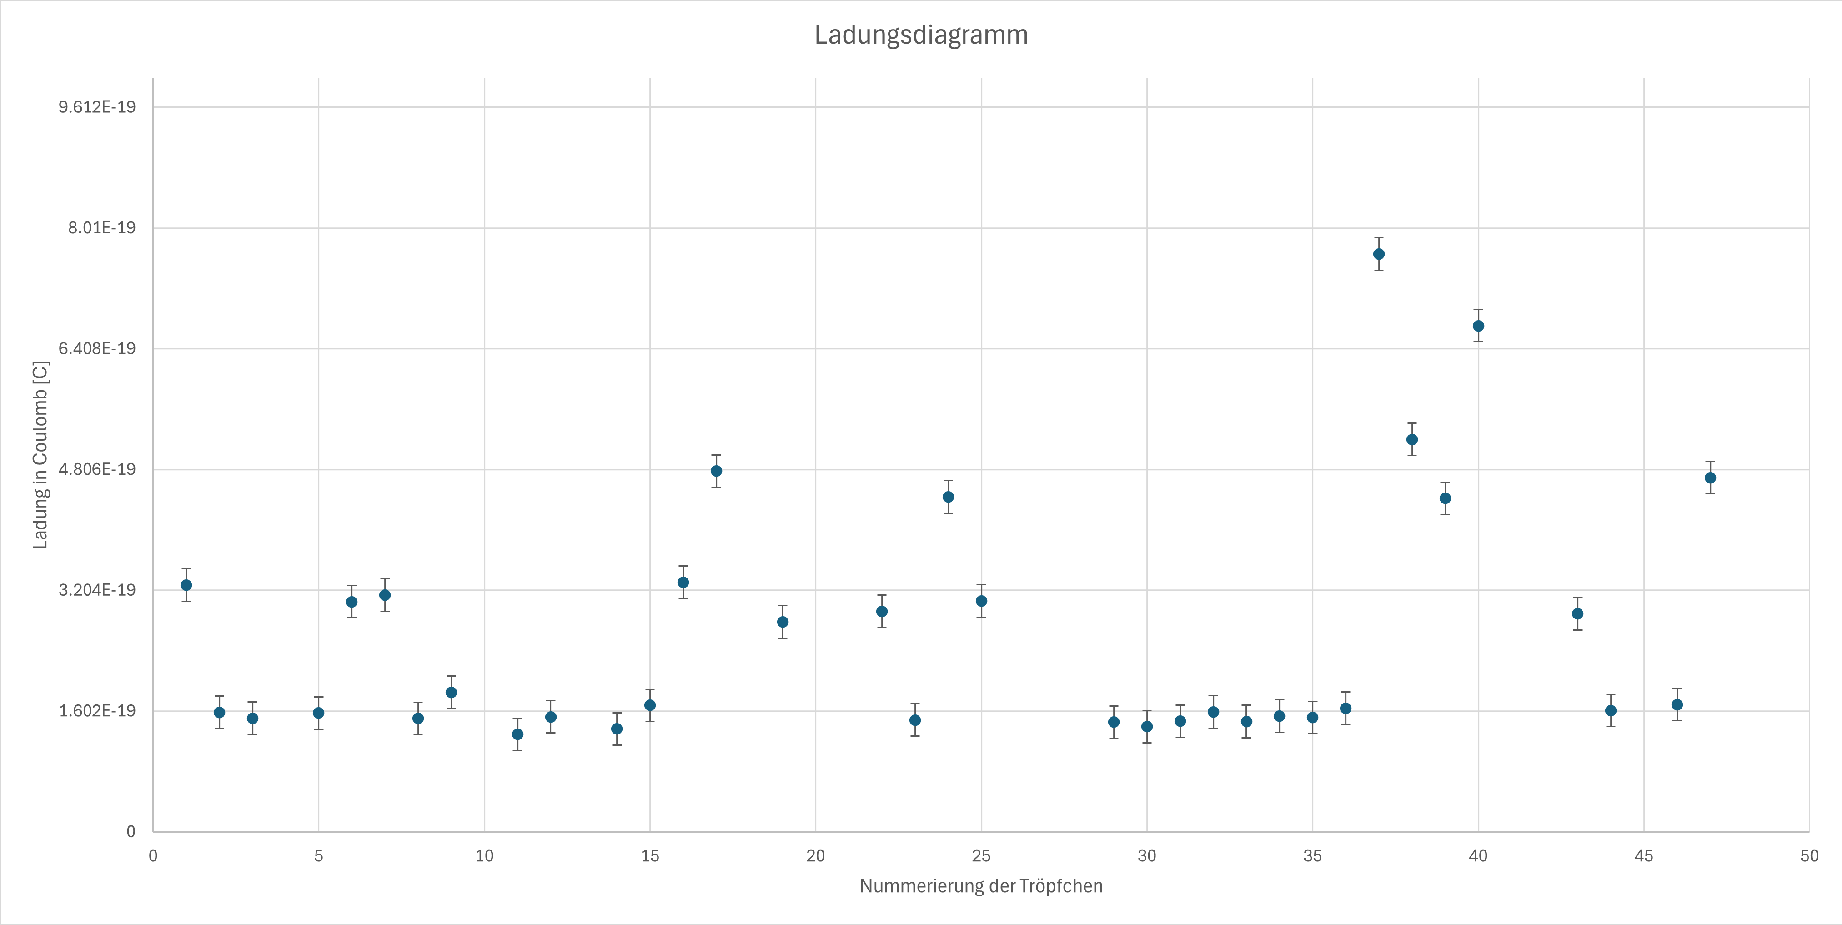
\includegraphics[width=\textwidth]{bilder/pdf/LadungsdiagrammMit.pdf}
	\caption{Ladungsdiagramm mit Fehlerrechnung}
	\label{fig:ladungsdiagrammMFehlerrechnung}
\end{figure}

\subsection{Schlussfolgerung des Ergebnis}\label{sub:schlussfolgerung}
Mit diesem Schritt wird das Ergebnis des Millikan-Versuchs vollständig abgeschlossen. Das Diagramm, das zusammen mit den Fehlerberechnungen erstellt wurde, zeigt deutlich, dass alle Tröpfchen einer bestimmten Ladungsstufe zugeordnet werden können. Dies war während des Experiments zunächst nicht absehbar. Es ist bemerkenswert, wie trotz der Vielzahl an Messgrößen, die alle mit verschiedenen Fehlerquellen behaftet sind, der berechnete Wert mit 19 Dezimalstellen konstant bleibt und sich im Bereich der theoretisch erwarteten Elementarladung bewegt. Dies verdeutlicht die hohe Präzision des Experiments und die Stabilität des Ergebnisses, auch bei der Auswertung der zahlreichen Messungen.



\begin{table}
\caption{Ergebnisse der Berechnung}
\label{tab:ergebnisse}
\begin{tabular}{lllll}
\toprule
v_rise & v_fall & Radius & Masse & Ladung \\
\midrule
2.01 \times 10^{-04} & 2.12 \times 10^{-05} & 4.04 \times 10^{-07} & 2.45 \times 10^{-16} & 3.27 \times 10^{-19} \\
8.46 \times 10^{-05} & 2.16 \times 10^{-05} & 4.08 \times 10^{-07} & 2.53 \times 10^{-16} & 1.59 \times 10^{-19} \\
8.68 \times 10^{-05} & 1.98 \times 10^{-05} & 3.90 \times 10^{-07} & 2.20 \times 10^{-16} & 1.51 \times 10^{-19} \\
8.91 \times 10^{-05} & 2.04 \times 10^{-05} & 3.96 \times 10^{-07} & 2.31 \times 10^{-16} & 1.58 \times 10^{-19} \\
1.97 \times 10^{-04} & 1.98 \times 10^{-05} & 3.89 \times 10^{-07} & 2.18 \times 10^{-16} & 3.05 \times 10^{-19} \\
1.98 \times 10^{-04} & 2.04 \times 10^{-05} & 3.96 \times 10^{-07} & 2.31 \times 10^{-16} & 3.14 \times 10^{-19} \\
9.33 \times 10^{-05} & 1.84 \times 10^{-05} & 3.74 \times 10^{-07} & 1.95 \times 10^{-16} & 1.50 \times 10^{-19} \\
1.26 \times 10^{-04} & 1.71 \times 10^{-05} & 3.61 \times 10^{-07} & 1.74 \times 10^{-16} & 1.85 \times 10^{-19} \\
1.12 \times 10^{-04} & 1.23 \times 10^{-05} & 3.01 \times 10^{-07} & 1.01 \times 10^{-16} & 1.29 \times 10^{-19} \\
1.30 \times 10^{-04} & 1.29 \times 10^{-05} & 3.08 \times 10^{-07} & 1.09 \times 10^{-16} & 1.53 \times 10^{-19} \\
1.26 \times 10^{-04} & 1.15 \times 10^{-05} & 2.89 \times 10^{-07} & 8.97 \times 10^{-17} & 1.37 \times 10^{-19} \\
1.21 \times 10^{-04} & 1.58 \times 10^{-05} & 3.45 \times 10^{-07} & 1.52 \times 10^{-16} & 1.68 \times 10^{-19} \\
2.26 \times 10^{-04} & 1.81 \times 10^{-05} & 3.72 \times 10^{-07} & 1.91 \times 10^{-16} & 3.31 \times 10^{-19} \\
4.50 \times 10^{-04} & 1.21 \times 10^{-05} & 2.97 \times 10^{-07} & 9.76 \times 10^{-17} & 4.79 \times 10^{-19} \\
2.84 \times 10^{-04} & 1.07 \times 10^{-05} & 2.76 \times 10^{-07} & 7.83 \times 10^{-17} & 2.79 \times 10^{-19} \\
2.43 \times 10^{-04} & 1.40 \times 10^{-05} & 3.23 \times 10^{-07} & 1.25 \times 10^{-16} & 2.93 \times 10^{-19} \\
1.26 \times 10^{-04} & 1.28 \times 10^{-05} & 3.07 \times 10^{-07} & 1.07 \times 10^{-16} & 1.48 \times 10^{-19} \\
3.97 \times 10^{-04} & 1.30 \times 10^{-05} & 3.10 \times 10^{-07} & 1.11 \times 10^{-16} & 4.44 \times 10^{-19} \\
2.49 \times 10^{-04} & 1.45 \times 10^{-05} & 3.29 \times 10^{-07} & 1.32 \times 10^{-16} & 3.06 \times 10^{-19} \\
3.96 \times 10^{-05} & 3.36 \times 10^{-05} & 5.20 \times 10^{-07} & 5.22 \times 10^{-16} & 1.46 \times 10^{-19} \\
1.04 \times 10^{-04} & 1.47 \times 10^{-05} & 3.31 \times 10^{-07} & 1.35 \times 10^{-16} & 1.40 \times 10^{-19} \\
5.22 \times 10^{-05} & 2.89 \times 10^{-05} & 4.79 \times 10^{-07} & 4.08 \times 10^{-16} & 1.47 \times 10^{-19} \\
5.40 \times 10^{-05} & 3.06 \times 10^{-05} & 4.95 \times 10^{-07} & 4.50 \times 10^{-16} & 1.59 \times 10^{-19} \\
5.82 \times 10^{-05} & 2.67 \times 10^{-05} & 4.59 \times 10^{-07} & 3.60 \times 10^{-16} & 1.46 \times 10^{-19} \\
5.34 \times 10^{-05} & 2.98 \times 10^{-05} & 4.88 \times 10^{-07} & 4.30 \times 10^{-16} & 1.54 \times 10^{-19} \\
5.76 \times 10^{-05} & 2.79 \times 10^{-05} & 4.71 \times 10^{-07} & 3.87 \times 10^{-16} & 1.52 \times 10^{-19} \\
5.81 \times 10^{-05} & 3.01 \times 10^{-05} & 4.91 \times 10^{-07} & 4.38 \times 10^{-16} & 1.64 \times 10^{-19} \\
5.32 \times 10^{-04} & 1.89 \times 10^{-05} & 3.81 \times 10^{-07} & 2.06 \times 10^{-16} & 7.67 \times 10^{-19} \\
3.55 \times 10^{-04} & 1.90 \times 10^{-05} & 3.82 \times 10^{-07} & 2.06 \times 10^{-16} & 5.21 \times 10^{-19} \\
3.31 \times 10^{-04} & 1.65 \times 10^{-05} & 3.54 \times 10^{-07} & 1.64 \times 10^{-16} & 4.42 \times 10^{-19} \\
4.85 \times 10^{-04} & 1.78 \times 10^{-05} & 3.68 \times 10^{-07} & 1.85 \times 10^{-16} & 6.71 \times 10^{-19} \\
2.10 \times 10^{-04} & 1.66 \times 10^{-05} & 3.55 \times 10^{-07} & 1.66 \times 10^{-16} & 2.89 \times 10^{-19} \\
1.04 \times 10^{-04} & 1.77 \times 10^{-05} & 3.67 \times 10^{-07} & 1.83 \times 10^{-16} & 1.61 \times 10^{-19} \\
2.14 \times 10^{-04} & 7.96 \times 10^{-06} & 2.34 \times 10^{-07} & 4.75 \times 10^{-17} & 1.69 \times 10^{-19} \\
6.02 \times 10^{-04} & 8.06 \times 10^{-06} & 2.36 \times 10^{-07} & 4.85 \times 10^{-17} & 4.70 \times 10^{-19} \\
\bottomrule
\end{tabular}
\end{table}

	\chapter{Fazit}\label{cha:fazit}
	
	
	
	
	
	\cleardoublepage
	\listoffigures
	\printbibliography
	\chapter{Eigenständigkeitserklärung}\label{cha:eigenständigkeitserklärung}
Ich bestätige mit meiner Unterschrift, dass ich meine Maturaarbeit selbständig verfasst und in schriftliche Form gebracht habe, dass sich die Mitwirkung anderer Personen auf Beratung und Korrekturlesen beschränkt hat und dass alle verwendeten Unterlagen und Gewährspersonen aufgeführt sind. Mir ist bekannt, dass eine Maturaarbeit, die nachweislich ein Plagiat gemäss Art. 1quater des Maturitätsprüfungsreglements des Gymnasiums (s. auch Maturaarbeitsbroschüre) darstellt, als schwerer Verstoss gewertet wird.
\vspace{1.5cm}

\noindent Datum und Unterschrift: \rule[-2mm]{11cm}{0.4pt} 
	
\end{document}





